%% ============================================================================
%%  UAGS: RA-L first submission (double-anonymous), RAS conference class.
%%  Assembled 2026-09-29 from the section drafts (front, related, method,
%%  experiments, preamble). Source of every claim: the 2026-09-29 fact sheet
%%  (docs/reports/2026-09-29-paper-revision-1/logs/fact_sheet.md); the code
%%  under usplat/ is the ground truth for every formula.
%%  Revised 2026-09-29 after the math, claims and form reviews (fix pass).
%%
%%  >>> READ ME BEFORE SUBMITTING <<<
%%  * Every number cell is a placeholder: \ph (XX.X), \phs (XX.X +- XX.X) or
%%    \phn (integer). These are NOT results. Search this file for \ph and \todo.
%%  * Localization and active view selection (EFE) are not part of this paper.
%%    Their old text is parked in papers/parked_sections.tex, as is the old
%%    timing table and the old fourth contribution (one backward pass).
%%  * Build: tectonic main.tex (runs BibTeX itself). References: ref.bib, plus
%%    ieeectl.bib, which the preamble writes on the first pass (et al. rule).
%% ============================================================================
%% Fonts under tectonic (tectonic runs XeTeX, not pdfLaTeX).
%% IEEEtran selects Times with \rmdefault{ptm}. XeTeX's default text encoding
%% is TU, and there is no TU/ptm font. Without the next line the text silently
%% falls back to Latin Modern and \bfseries prints in regular weight.
%% T1 selects the URW Times Type 1 fonts (NimbusRomNo9L) that pdfLaTeX uses
%% for the reference PDF. It must come BEFORE \documentclass: the class
%% sets its display and paragraph skips in ex units while it loads, so it must
%% see Times then, as it does under pdfLaTeX (loaded later, these skips come
%% out about 4% too small).
%% Keep the .tex and .bib sources ASCII. Write accents as LaTeX commands
%% (e.g. {\'e}) and quotes as ``...''. T1 under XeTeX does not map Unicode
%% input: a typed curly quote prints as a wrong glyph.
\RequirePackage[T1]{fontenc}

%% RA-L is a JOURNAL, so the submission uses the IEEE journal template.
%% (This file briefly used ieeeconf, the ICRA/IROS conference class; that was
%% wrong for RA-L. \overrideIEEEmargins and \IEEEoverridecommandlockouts were
%% ieeeconf/conference-mode commands and are gone with it.)
\documentclass[journal]{IEEEtran}

%% ---------------------------------------------------------------------------
%% Packages
%% ---------------------------------------------------------------------------
\usepackage{amsmath,amssymb,amsfonts}
\interdisplaylinepenalty=2500 % IEEEtran advice after amsmath: lets align break pages
\usepackage{graphicx}
\usepackage{booktabs}
\usepackage{array}
\usepackage{textcomp}         % \textdegree and similar text symbols
\usepackage{algorithm}        % float wrapper for pseudo-code
\usepackage{algorithmic}      % \begin{algorithmic} ... \STATE ...
\usepackage{xcolor}
\usepackage{cite}             % sorted, compressed numeric citations [1]-[3]
%% amsthm clashes with ieeeconf: the class already defines \proof and
%% \endproof, so \usepackage{amsthm} stops with "Command \proof already
%% defined". If amsthm is ever needed, load it like this:
%\let\proof\relax
%\let\endproof\relax
%\usepackage{amsthm}
%% ieeeconf has its own \newtheorem style, so plain \newtheorem works without amsthm.
\usepackage[colorlinks=true,allcolors=blue]{hyperref}  % load hyperref last
\hypersetup{pdfauthor={Anonymous Authors}}             % keep PDF metadata anonymous

%% IEEE reference style: at most 6 authors, then "et al.". IEEEtran.bst reads
%% the control entry IEEEexample:BSTcontrol from ieeectl.bib through
%% \bstctlcite, which IEEEtran.cls provides. The file is
%% written here on the first pass only (a marker in main.aux skips it later),
%% so tectonic does not rerun TeX for a rewritten ieeectl.bib. Delete main.aux
%% to regenerate it.
\makeatletter
\newwrite\uags@ctl
\AtBeginDocument{%
  \@ifundefined{uags@ctldone}{%
    \immediate\openout\uags@ctl=ieeectl.bib\relax
    \immediate\write\uags@ctl{\@percentchar\space IEEEtran.bst control entry, written by main.tex}%
    \immediate\write\uags@ctl{@IEEEtranBSTCTL\@charlb IEEEexample:BSTcontrol,}%
    \immediate\write\uags@ctl{\space\space CTLuse_forced_etal = "yes",}%
    \immediate\write\uags@ctl{\space\space CTLmax_names_forced_etal = "6",}%
    \immediate\write\uags@ctl{\space\space CTLnames_show_etal = "1"}%
    \immediate\write\uags@ctl{\@charrb}%
    \immediate\closeout\uags@ctl}{}%
  \immediate\write\@auxout{\gdef\string\uags@ctldone{}}}
\makeatother
%% \bstctlcite comes from IEEEtran.cls, so it is not defined here any more.

%% ---------------------------------------------------------------------------
%% Draft macros (same as papers/main.tex)
%% ---------------------------------------------------------------------------
\newcommand{\todo}[1]{\textcolor{red}{\textbf{[TODO: #1]}}}
\newcommand{\ph}{\textcolor{red}{XX.X}}      % numeric placeholder
\newcommand{\phn}{\textcolor{red}{X}}        % integer placeholder
\newcommand{\R}{\mathbf{R}}
\newcommand{\xv}{\mathbf{x}}
\newcommand{\zv}{\mathbf{z}}
\newcommand{\muv}{\boldsymbol{\mu}}
\newcommand{\etav}{\boldsymbol{\eta}}
\newcommand{\Sph}{\mathbb{S}}
\newcommand{\reimpl}{\textsuperscript{$\dagger$}}   % re-implemented baseline row
\newcommand{\phs}{\ph{\scriptsize$\,\pm\,$\ph}}     % mean +- std placeholder
\newcommand{\secref}[1]{Sec.~\mbox{\ref{#1}}}       % keeps "III-F" on one line

%% ---------------------------------------------------------------------------
%% Title and anonymous byline (double-anonymous: no names, affiliations,
%% e-mails, funding, \thanks notes or acknowledgments)
%% ---------------------------------------------------------------------------
%% Title. The plan (2026-09-28-paper-completion-plan/1-plan.md, Sec. 6) ties the title to
%% the G2 grid; this is cell A. Swap once G2/G3 are measured:
%%   B (epistemic pass, calibration fail): Detecting and Forgetting Stale Open-Vocabulary
%%     Semantics in Gaussian Splatting with View-Level Evidence
%%   C (epistemic fail, calibration pass): Calibrated Open-Vocabulary Gaussian Splatting
%%     that Forgets Stale Semantics
%%   D (both fail): Detecting and Forgetting Stale Open-Vocabulary Semantics in Gaussian
%%     Splatting
\title{Uncertainty-Aware Open-Vocabulary Gaussian Splatting for Changing Scenes}

%% Double-anonymous review: no names, affiliations, funding or links.
\author{Anonymous Authors}

%% Notes (from the template check):
%%  * IEEEtran provides IEEEkeywords and \IEEEPARstart. RA-L collects the
%%    keywords in the PaperCept form as well, so the block is optional for
%%    the first submission.
%%  * Last page: to balance the columns, put \addtolength{\textheight}{-Xcm}
%%    in the text of the last page (tune X by hand), as the official root.tex does.

\begin{document}
\bstctlcite{IEEEexample:BSTcontrol}

\maketitle
%% Page numbers are left ON: reviewers refer to them. (ieeeconf's
%% \pagestyle{empty} lines were removed with that class.)

%% ----------------------------------------------------------------------------
\begin{abstract}
A robot that reuses a semantic map must know how much evidence supports each
part, and must stop trusting content that has changed. We present a
probabilistic open-vocabulary field for 3D Gaussian Splatting that serves both
needs. Each Gaussian holds a von Mises--Fisher posterior over the direction of
its vision-language feature. Each keyframe counts as at most one observation
per Gaussian, because the pixels of one view are strongly correlated. The same
sufficient statistics give an epistemic uncertainty, from the weighted number
of views, and an aleatoric uncertainty, from a bias-corrected agreement of the
views. Little evidence and conflicting evidence thus stay separate. We detect
change with a known feature residual and set its threshold per scene, without
labels, from the map's own mapping pass. A Gaussian that fails the test is
reset. When depth is available, it rejoins the robust map only after new views
whose observed depth matches its position. A posterior predictive turns the
field into per-pixel class probabilities. We evaluate on Replica and on 16
real scenes from which an object was physically removed.
%% Headline sentence: at most ~20 words (the rest is about 170 words; limit 200).
\todo{headline result}
\end{abstract}

%% RAS keyword list, 2-5 terms, no localization.
\begin{IEEEkeywords}
Semantic Scene Understanding, Mapping, Probability and Statistical Methods,
RGB-D Perception
\end{IEEEkeywords}

%% ============================================================================
\section{Introduction}
%% ============================================================================
Robots in homes and offices increasingly query their maps with
language~\cite{lee2026lamp, nagami2025vista}.
Open-vocabulary 3D Gaussian Splatting (3D-GS)~\cite{kerbl2023} supports such
queries by attaching vision-language features~\cite{radford2021} to the
Gaussians of the map~\cite{qin2024langsplat, zhou2024feature,
wu2024opengaussian, shi2024legaussians}. A robot that reuses the map needs more
than the most likely label. It needs to know how much evidence stands behind
each Gaussian's semantics, whether that evidence agrees, and whether it is
still valid. Indoor scenes change. Objects are moved or removed, and a map that
keeps their old semantics answers queries with content that is no longer
there.

%% Fig. 1. Placed after the first paragraph so that the float cannot land
%% above the abstract. "Calibration" is not used in the figure or the caption
%% (fact sheet C: "calibrated" only for the predictive).
\begin{figure*}[t]
  \centering
  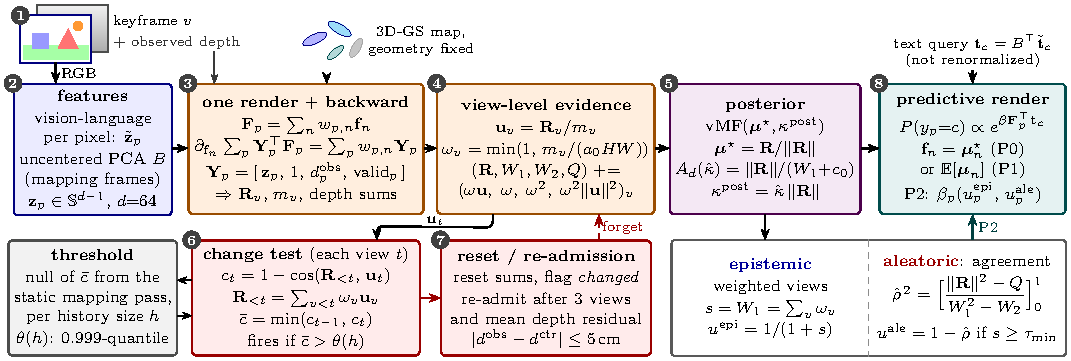
\includegraphics[width=\textwidth]{figs/pipeline.pdf}
  \caption{One keyframe update. (1)~A posed keyframe gives RGB and, when
  available, observed depth. (2)~Dense vision-language features, compressed by
  a PCA fit on the mapping frames. (3)~One render and one backward
  pass~\cite{joseph2025gradbp} give every Gaussian its per-view sums. (4)~Each
  view is one observation $\mathbf{u}_v$ with weight $\omega_v$. (5)~Four
  running sums give the vMF posterior, the support $s$ and the agreement
  $\hat\rho$. (6)~A change test with a threshold $\theta(h)$ from the static
  mapping pass. (7)~Reset, and re-admission after a depth check. (8)~A
  predictive render answers text queries. The index $n$ is dropped.}
  \label{fig:pipeline}
\end{figure*}

Several works attach uncertainty to such maps. Bayesian Kernel Inference
(BKI)~\cite{vegabrown2014, gan2020bayesian} fuses kernel-weighted observations
in closed form, and Continuous Semantic Splatting (CSS)~\cite{wilson2025css}
brings it to 3D-GS with a Dirichlet posterior over a fixed label set. Other
work fuses open-set features on voxels~\cite{wilson2025latentbki}, learns an
uncertainty~\cite{shi2024legaussians, lee2026lamp}, or scores the reliability
of lifted features~\cite{zang2026normlift}. These methods assume a static
scene. Change-aware maps~\cite{lu2025gscd, ackermann2025clsplats,
zeng2025gaussianupdate, he2026vgmapping, jiang2026mif} detect moved or removed
content by comparing new observations with the map. Two questions fall
between these lines of work: how a detected change should enter the
uncertainty bookkeeping, and how to set the detection threshold on a new scene
without labels.

We answer both questions inside one Bayesian field. Each Gaussian holds a vMF
posterior~\cite{mardia2000directional} over the direction of its feature. A
keyframe contributes one weighted observation per Gaussian: the splat-weighted
mean of the pixel features that the Gaussian covers. To detect change, we
compare all earlier evidence of a Gaussian with the current view. This
statistic is the classic feature residual~\cite{ackermann2025clsplats,
jiang2026mif}, and we do not claim it as new. Our part is what happens around
it: how the threshold is set without labels, which evidence is reset, and when
a Gaussian is trusted again. Geometry stays fixed after mapping, so moved
content is forgotten at its old place but not inserted at its new one.
Fig.~\ref{fig:pipeline} shows one keyframe update. Our contributions are:
\begin{itemize}
\item \textbf{A directional posterior with view-level evidence.} Each Gaussian
keeps a vMF posterior, the directional counterpart of Dirichlet semantic
mapping, that receives one weighted observation per view. Its epistemic
read-out is the weighted number of views. Its aleatoric read-out is a
bias-corrected agreement of the views that does not shrink with the amount of
evidence.
\item \textbf{Change handling in the Bayesian bookkeeping.} The threshold of
the residual is a quantile of the map's own mapping-pass scores, per history
length. This targets a nominal per-view false-alarm rate on static content
without labels, and we measure the actual rate. A flagged Gaussian is reset
and rejoins the robust map only after a depth check.
\item \textbf{A predictive that uses both uncertainties.} Each pixel's
temperature depends on its rendered epistemic and aleatoric uncertainties. We
test whether this, or a render of each Gaussian's posterior mean feature,
lowers NLL and ECE compared with plug-in features at their own fitted
temperature.
\end{itemize}

We evaluate segmentation, uncertainty ranking and calibration on 8 Replica
scenes~\cite{straub2019replica, zhi2021semanticnerf}, and stale-content
detection on 16 real scenes in which an object was physically
removed~\cite{weder2023removing}. \todo{one sentence on the main measured
finding.}

%% ============================================================================
%% Related Work
%% ============================================================================
\section{Related Work}
\label{sec:related}

\textbf{Language-embedded 3D-GS.}
LangSplat~\cite{qin2024langsplat}, Feature 3DGS~\cite{zhou2024feature},
OpenGaussian~\cite{wu2024opengaussian} and LEGaussians~\cite{shi2024legaussians}
optimize per-Gaussian features through rendering against 2D foundation-model
features or masks. LEGaussians also learns a per-Gaussian uncertainty.
Training-free methods~\cite{cheng2025occam, joseph2025gradbp} give each
Gaussian the splat-weighted average of its pixel features,
which~\cite{joseph2025gradbp} reads from the gradient of one render. The
concurrent NormLift~\cite{zang2026normlift} averages per-view mean features.
It factors the norm of the un-normalized mean into within-view and cross-view
consistency. On static scenes it scores reliability by that norm, shrunk by a
Kish count~\cite{kish1965survey} of effective views. We reuse the gradient
identity and NormLift's per-view mean. We differ in three ways. Our cross-view
agreement is bias-corrected and does not shrink with the amount of evidence.
It enters a vMF posterior with a predictive whose calibration we test. We also
handle scene change.

\textbf{Probabilistic semantic mapping.}
BKI~\cite{vegabrown2014} updates a conjugate
posterior with kernel-tempered observations. Semantic BKI~\cite{gan2020bayesian}
keeps a Dirichlet posterior over classes in voxels, and
E2-BKI~\cite{kim2025e2bki} adds evidential reasoning and ellipsoidal kernels.
CSS~\cite{wilson2025css} brings the Dirichlet model to 3D-GS with the splat
weight as the kernel. It separates sparse from conflicting observations over a
closed label set fixed at mapping time, and names an open-dictionary conjugate
prior as future work. LatentBKI~\cite{wilson2025latentbki} and
SLIM-VDB~\cite{sheppard2026slimvdb} fuse open-set features on voxels under
Gaussian models. Bayesian Fields~\cite{maggio2025bayesian} updates
per-Gaussian relevance probabilities for tasks given at mapping time.
PhysGS~\cite{chopra2026physgs} splits aleatoric from epistemic
variance~\cite{kendall2017uncertainties} for physical properties in 3D-GS. We
start from the splat-weight kernel of CSS, normalize it per view, and model
unit features with a vMF distribution (\secref{sec:posterior}).

\textbf{Directional statistics.}
The vMF distribution is the standard model for unit
vectors~\cite{mardia2000directional}. Its mean direction has a conjugate vMF
prior~\cite{mardia1976bayesian}, and vMF mixtures cluster high-dimensional unit
vectors~\cite{banerjee2005vmf}. The implicit language field of
LAMP~\cite{lee2026lamp} outputs a vMF mean and a concentration, read as
aleatoric uncertainty. We train no network. Each Gaussian keeps additive
sufficient statistics instead.

\textbf{Change detection and long-term maps.}
3DGS-CD~\cite{lu2025gscd} finds rearranged objects from render-image
differences and segmentation masks. CL-Splats~\cite{ackermann2025clsplats}
compares DINOv2 features of renders and images, then re-optimizes only changed
regions. GaussianUpdate~\cite{zeng2025gaussianupdate} uses continual learning
with generative replay, and VG-Mapping~\cite{he2026vgmapping} adds and removes
Gaussians in changed regions of semi-static scenes. MIF~\cite{jiang2026mif}
updates its scene memory where the discrepancy of matched scene-graph nodes, a
position term plus a feature-cosine term, exceeds a fixed threshold. Chu and
Kim~\cite{chu2026semantic} let a language model pick stable objects to
localize in changing indoor scenes. Our change score is the same kind of
feature residual as that of CL-Splats and the semantic term of MIF. It is one
minus the cosine between all earlier evidence of a Gaussian and the current
view, and a change must persist over two views. We differ in the threshold and
the response. The threshold is a quantile of the map's own mapping-pass scores
per history size, so it needs no labels. A detection resets the Gaussian's
semantic evidence, and new views with a depth check gate its return. Unlike
CL-Splats, GaussianUpdate and VG-Mapping, we keep geometry fixed.

%% ============================================================================
\section{Method}
\label{sec:method}
%% ============================================================================
%% Symbols: w_{p,n} = splat weight, \omega_{v,n} = view weight, \lambda = retention
%% of the change test (fact sheet "beta"), \beta = temperature of the predictive,
%% k = persistence window, M = number of mapping frames (Sec. metrics),
%% \gamma_e, \gamma_a, \gamma_u = P2 coefficients (code: a, b, g).
Each keyframe gives every visible Gaussian one view-level observation, and a
few running sums hold its semantic state (Fig.~\ref{fig:pipeline},
Alg.~\ref{alg:update}).

\subsection{Preliminaries}
\label{sec:prelim}
The map holds $N$ Gaussians~\cite{kerbl2023}, and its geometry is fixed after
mapping. At pixel $p$, Gaussian $n$ has opacity $\alpha_{p,n}$: its base opacity
times its projected 2D Gaussian evaluated at $p$. With the Gaussians sorted by
depth, the splat weight is $w_{p,n}=T_{p,n}\,\alpha_{p,n}$ with the
transmittance $T_{p,n}=\prod_{j<n}(1-\alpha_{p,j})$. It is the share of pixel
$p$ that Gaussian $n$ explains. A per-Gaussian buffer $\mathbf{f}_n$ renders
to $\mathbf{F}_p=\sum_n w_{p,n}\mathbf{f}_n$, and $\alpha_p=\sum_n
w_{p,n}\le1$ is the rendered opacity. As in CSS~\cite{wilson2025css},
$w_{p,n}$ is the BKI kernel~\cite{vegabrown2014, gan2020bayesian}.

\subsection{Features and Query Space}
\label{sec:features}
A dense extractor, LSeg~\cite{li2022lseg}, gives unit pixel features
$\tilde\zv_p$ that are cosine-comparable with unit CLIP text embeddings
$\tilde{\mathbf{t}}_c$~\cite{radford2021}. An uncentered PCA with orthonormal
basis $B$, fit on mapping frames only (no text, no labels), compresses them to
$d=64$: $\zv_p=B^\top\tilde\zv_p/\lVert B^\top\tilde\zv_p\rVert\in\Sph^{d-1}$.
Texts are projected without renormalization,
$\mathbf{t}_c=B^\top\tilde{\mathbf{t}}_c$, so
$\muv^\top\mathbf{t}_c=(B\muv)^\top\tilde{\mathbf{t}}_c$ is the full-space
cosine between the decoded direction $B\muv$ and the text. Renormalizing
$\mathbf{t}_c$ would inflate texts with little energy in the image subspace
and can change the argmax label.

\subsection{View-Level Evidence}
\label{sec:evidence}
Keyframe $v$ gives every Gaussian $n$ the sums $\R_{v,n}=\sum_p w_{p,n}\zv_p$ and
$m_{v,n}=\sum_p w_{p,n}$. We read them from one render and one backward
pass. With geometry and opacity detached, $\mathbf{F}_p$ is linear in the
buffer, so the gradient of $\sum_p\mathbf{Y}_p^\top\mathbf{F}_p$ with respect
to $\mathbf{f}_n$ is $\sum_p w_{p,n}\mathbf{Y}_p$ for any per-pixel target
$\mathbf{Y}_p$. We take this identity from Gradient-Weighted Feature
Back-Projection~\cite{joseph2025gradbp}, and stack $\zv_p$, a ones channel and
the observed depth with its validity mask into one target. This gives all
per-Gaussian sums of Alg.~\ref{alg:update}, with no per-Gaussian pixel lists.
It needs a rasterizer affine in per-Gaussian features. We use gsplat~\cite{ye2024gsplat}
with the buffer in place of the colors and no spherical harmonics.

Pixels of one view are strongly correlated. For example, one ViT-L/16 patch of LSeg covers
$16\times16$ pixels. A pixel count thus overstates the evidence and grows with
the image resolution, so we count views. View $v$ gives Gaussian $n$ one
observation, the view mean $\mathbf{u}_{v,n}=\R_{v,n}/m_{v,n}$, as in
NormLift~\cite{zang2026normlift}. Its length $\lVert\mathbf{u}_{v,n}\rVert\le1$
is the coherence inside the view. Its weight
$\omega_{v,n}=\min(1,\,m_{v,n}/(a_0HW))$ (default $a_0=10^{-4}$) does not depend
on the resolution, and a view with a smaller footprint counts fractionally.
Gaussian $n$ keeps four sums over its views, written without the indices on
the right:
\[
\R_n=\textstyle\sum\omega\mathbf{u},\;
W_1=\sum\omega,\;
W_2=\sum\omega^2,\;
Q=\sum\omega^2\lVert\mathbf{u}\rVert^2 .
\]

\subsection{Direction Posterior and Concentration}
\label{sec:posterior}
We use a vMF likelihood
$p(\zv\mid\muv,\kappa)=C_d(\kappa)\,e^{\kappa\muv^\top\zv}$ on
$\Sph^{d-1}$~\cite{mardia2000directional, banerjee2005vmf}. Following BKI, we
temper the likelihood of pixel $p$ in view $v$ by the kernel
$\omega_{v,n}w_{p,n}/m_{v,n}$. A view
then carries mass $\omega_{v,n}$ and log-likelihood
$\omega_{v,n}\big(\log C_d(\kappa)+\kappa\muv^\top\mathbf{u}_{v,n}\big)$. Given
$\kappa_n$, the direction posterior is a vMF~\cite{mardia1976bayesian} with
natural parameter $\etav_n=\kappa_n\R_n+\kappa_0\muv_0$, mean direction
$\muv^\star_n=\etav_n/\lVert\etav_n\rVert$ and concentration
$\kappa^{\mathrm{post}}_n=\lVert\etav_n\rVert$. The optional text prior is off
($\kappa_0=0$), so $\muv^\star_n=\R_n/\lVert\R_n\rVert$. For $\kappa_n$ we use
the joint conjugate prior
$p(\muv,\kappa)\propto C_d(\kappa)^{c_0}e^{\kappa\mathbf{m}_0^\top\muv}$ with
$\mathbf{m}_0=\mathbf{0}$ (default $c_0=1$). The joint posterior is
proportional to $C_d(\kappa)^{W_1+c_0}e^{\kappa\muv^\top\R_n}$, and its MAP
concentration solves
\begin{equation}
A_d(\hat\kappa_n)=\frac{\lVert\R_n\rVert}{W_1+c_0},\qquad
A_d(\kappa)=\frac{I_{d/2}(\kappa)}{I_{d/2-1}(\kappa)},
\label{eq:kappa}
\end{equation}
where $A_d(\kappa)=\mathbb{E}[\muv^\top\zv]$ is the mean cosine of a vMF. We set
$\kappa_n=\hat\kappa_n$, so $\kappa^{\mathrm{post}}_n=\hat\kappa_n\lVert\R_n\rVert$.
The concentration never changes $\muv^\star_n$ or the label. It only sets how
sharp the posterior is. With one-hot features, $\R_n$ equals the count
increment of categorical BKI run with our view-level kernel.
(CSS~\cite{wilson2025css} uses the pixel kernel $w_{p,n}$, so its counts
differ.) The two models share the sufficient statistic and the MAP label but
not the distribution, so the vMF model is the directional counterpart of
Dirichlet semantic mapping.

\subsection{Epistemic and Aleatoric Uncertainty}
\label{sec:uncertainty}
\textbf{Epistemic.} The support $s_n=W_1$ is the number of views, each
weighted by $\omega\le1$, and $u^{\mathrm{epi}}_n=1/(1+s_n)$. Because
$\omega\le1$, the Kish effective number of views~\cite{kish1965survey}
$n_K=W_1^2/W_2$ is never below $W_1$. It ignores the scale of the weights, so
it would count ten small partial views as much as ten full ones.

\textbf{Aleatoric.} Let $\rho_n=\lVert\mathbb{E}\,\mathbf{u}_{v,n}\rVert$. It is
one when every view shows the same unit feature and near zero when the views
disagree. We estimate it by
\begin{equation}
\hat\rho_n^2=\Big[\frac{\lVert\R_n\rVert^2-Q}{W_1^2-W_2}\Big]_0^1,\qquad
u^{\mathrm{ale}}_n=1-\hat\rho_n ,
\label{eq:rho}
\end{equation}
where $[\cdot]_0^1$ clamps to $[0,1]$. For independent views with a common
mean, the expected squared norm is $\mathbb{E}\lVert\R_n\rVert^2=(W_1^2-W_2)\rho_n^2+\sum_v\omega^2\,
\mathbb{E}\lVert\mathbf{u}_{v,n}\rVert^2$. The ratio inside the clamp is thus
unbiased for $\rho_n^2$ for two or more views. The clamp and the square root
leave a small bias at few views. The aleatoric uncertainty is defined once
$s_n\ge\tau_{\min}$ (default 3 views).%
%% Footnote source: docs/reports/2026-09-29-replica-tab1/logs/support_stats.log
%% (validation fields at code 5e8c51e; 640x480 frames, --downscale 2 in
%% scripts/replica_tab1.sh, so H*W = 320*240 and a0*H*W = 7.68 px).
\footnote{One full view is $a_0HW=7.68$ pixels of splat mass at our
$320\times240$ resolution. On office\_0 / room\_2, $u^{\mathrm{ale}}$ is
defined for 22.4 / 12.2\% of the Gaussians but 84.2 / 81.8\% of the pixel
mass.} Two simpler estimates mix the amount of
evidence into the dispersion. The mean resultant length
$\bar r_n=\lVert\R_n\rVert/W_1$ is biased upward, by up to about
$1/\sqrt{n_K}$. A prior-shrunk agreement such as $\lVert\R_n\rVert/(W_1+c_0)$
is small whenever evidence is scarce. NormLift's reliability, its feature norm
times $N_{\mathrm{eff}}/(N_{\mathrm{eff}}+1)$~\cite{zang2026normlift}, has this
form. Estimator~\eqref{eq:rho} removes the leading bias of $\bar r_n$ and does
not shrink, so little evidence and conflicting evidence stay separate
(Fig.~\ref{fig:plane}). The shrunk form suits $\hat\kappa_n$
in~\eqref{eq:kappa}, where scarce evidence should broaden the posterior.

\begin{figure}[t]
  \centering
  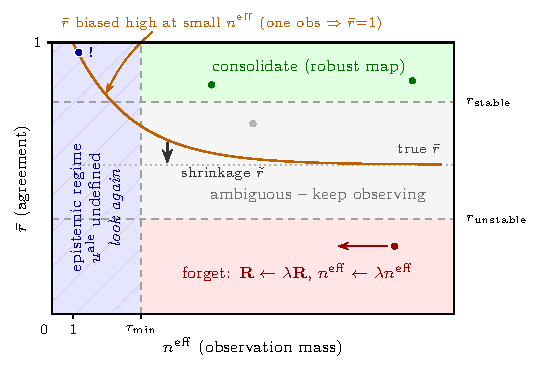
\includegraphics[width=\linewidth]{figs/uncertainty_plane.pdf}
  \caption{Support $s$ (weighted views) against agreement $\hat\rho$ of one
  Gaussian. The curves are root-mean-square values for two Gaussians with true
  agreement $\rho$ (dotted). The mean length $\lVert\R\rVert/W_1$ makes the
  conflicting one look consistent at few views, and the shrunk
  $\lVert\R\rVert/(W_1+c_0)$ makes the consistent one look conflicting. Our
  $\hat\rho$ is drawn at $\rho$: before the clamp $\hat\rho^2$ is unbiased, so
  $\hat\rho$ stays close to $\rho$. A fired change test resets $s$ to at most
  one view.}
  \label{fig:plane}
\end{figure}

\subsection{Change Detection, Reset and Re-admission}
\label{sec:change}
We test each Gaussian at each view with a family of two-bucket statistics. An
older bucket $\R^{\mathrm{old}}_n$ and a recent bucket $\R^{\mathrm{new}}_n$
split $\R_n$ without overlap. The test counts a view by
$\nu_{v,n}=m_{v,n}/\max_{v'\le v}m_{v',n}$, its share of the largest splat mass
the Gaussian has had so far, not by $\omega_{v,n}$. In a dense map most
Gaussians never cover $a_0HW$ pixels in one view, so a test on full views would
rarely run; we chose $\nu$ on the validation scenes (\secref{sec:setup}). Each
view moves a share $1-\lambda^{\nu}$ of the recent bucket, and of its mass,
into the older one. It then adds $\nu_{v,n}\mathbf{u}_{v,n}$ to the recent one
(retention $\lambda\in[0,1)$ per unit of $\nu$). The score
$c_n=1-\cos(\R^{\mathrm{old}}_n,\R^{\mathrm{new}}_n)$ is defined once the
buckets hold $\tau_{\min}$ views of weight $\nu$ and each holds at least half a
view. A change
must persist, so the statistic $\bar c_n$ is the minimum of the last $k$
defined scores.

%% Tuning scene: usplat/vmf_field.py:44 ("k = 2 won the chess grid") and
%% docs/reports/2026-09-29-data-and-baselines/README.md ("chess = tuning").
%% The tuning data are a point-level replay (scripts/cpu_check_change.py):
%% dense CLIP features of 3D points, the CHANGED half of the points take a
%% partner's features (> 0.5 m away) in the last half (or fifth, grid of
%% data-and-baselines attempts/03) of their views. No objects are swapped.
We chose $\lambda=0$ and $k=2$ on a tuning replay not used for testing: in
7-Scenes chess~\cite{glocker2013}, half of the sampled 3D points take the
CLIP features of a point over 0.5\,m away in their later views. Then
$\bar c_n$ is the minimum over the last two views $t$ of
$1-\cos\big(\sum_{v<t}\omega_{v,n}\mathbf{u}_{v,n},\,\mathbf{u}_{t,n}\big)$,
all earlier evidence against the current view. This member is the classic
feature-residual test~\cite{jiang2026mif, ackermann2025clsplats}, which we do
not claim. Centering the features on the scene mean hurt in tuning, so it is
off.

%% Fixed threshold, valid features: static c_max q0.95 = 0.273 (chess) vs
%% 0.202 (office), data-and-baselines logs/g1_{chess,office}_final_frac0.5.json
%% (the method-completion numbers used the broken extractor).
\textbf{Threshold from the mapping pass.} In tuning, a fixed threshold on
$\bar c_n$ did not transfer between scenes (fixed-threshold row of
Table~\ref{tab:ablation}). We therefore set it, without labels, from the map's
own mapping pass. That sequence is assumed static, so its scores sample the
no-change null (no resets happen during mapping). Short histories give noisier
scores, so we keep one null histogram per history size, the mass
$h_n=W^{\mathrm{old}}_n$ of the older bucket, with bin edges at 4, 6, 10, 20
and 40 views. The threshold $\theta(h)$ is the $q$-quantile of bin $h$
(default $q=0.999$), a nominal per-view false-alarm rate of $10^{-3}$ on static
content. A bin with fewer than 200 samples borrows the nearest bin with
enough. In tuning, a null of per-Gaussian maxima over the mapping pass was
inflated by the short early histories.

%% Re-admission as implemented (usplat/vmf_field.py:442-475): views_since_reset
%% restarts at 0 and then adds the omega of the view that fired, and the depth
%% record includes that view. The fact sheet's "3 new views" differs from this.
\textbf{Reset and re-admission.} When $\bar c_n>\theta(h_n)$, Gaussian $n$
forgets. Its four sums, buckets and depth record restart from the current
view, and it is flagged \emph{changed}. It is re-admitted at the first view at
which its weight $\nu$ since the reset, the view that fired included, is at
least 3 and the view-weighted mean of
$\lvert d^{\mathrm{obs}}_{v,n}-d^{\mathrm{ctr}}_{v,n}\rvert$ over these views
is at most 5\,cm. Here $d^{\mathrm{obs}}_{v,n}$ is the observed depth (sensor
or estimator, never rendered from the map) averaged over the footprint with
the weights $w_{p,n}$, and $d^{\mathrm{ctr}}_{v,n}$ is the camera depth of the
Gaussian center. The Gaussians of a removed object see the surface behind
them. They stay out while that surface lies more than 5\,cm from their
centers. A Gaussian with no valid depth since its reset stays out. Without any
depth stream, the views alone decide. The \emph{robust set} holds the
Gaussians with $s_n\ge\tau_{\min}$, $\hat\rho_n\ge0.6$ and no change flag.

\begin{algorithm}[t]
\caption{Update of the field with keyframe $v$}
\label{alg:update}
\begin{algorithmic}[1]
\STATE Render and backward pass: $\R_{v,n}$, $m_{v,n}$, depth sums
\FORALL{Gaussians $n$ with $m_{v,n}>0$, in parallel}
\STATE $\mathbf{u}\leftarrow\R_{v,n}/m_{v,n}$,\;
$\omega\leftarrow\min(1,m_{v,n}/(a_0HW))$,\;
$\nu\leftarrow m_{v,n}/\max_{v'\le v}m_{v',n}$
\STATE $\R^{\mathrm{old}}_n\mathrel{+}=(1-\lambda^{\nu})\R^{\mathrm{new}}_n$,\;
$\R^{\mathrm{new}}_n\leftarrow\lambda^{\nu}\R^{\mathrm{new}}_n+\nu\mathbf{u}$
\STATE If defined, $\bar c_n\leftarrow$ minimum of the last $k$ scores $c_n$.
While mapping, add $\bar c_n$ to the null of bin $h_n$. Later, reset and flag
$n$ if $\bar c_n>\theta(h_n)$.
\STATE $\R_n\mathrel{+}=\omega\mathbf{u}$, $W_1\mathrel{+}=\omega$,
$W_2\mathrel{+}=\omega^2$, $Q\mathrel{+}=\omega^2\lVert\mathbf{u}\rVert^2$
\STATE Update the depth residual, unflag $n$ if re-admitted
\ENDFOR
\STATE After mapping: $\theta(h)\leftarrow q$-quantile of the null of bin $h$
\end{algorithmic}
\end{algorithm}

\subsection{Predictive Distribution}
\label{sec:predictive}
For pixel $p$ of a novel view, the class probabilities are
\[
P(y_p=c)=\operatorname{softmax}_c\big(\beta\,\mathbf{F}_p^\top\mathbf{t}_c\big),
\qquad \mathbf{F}_p=\textstyle\sum_n w_{p,n}\mathbf{f}_n .
\]
The render $\mathbf{F}_p$ is not divided by $\alpha_p$, so low opacity
flattens the distribution. \emph{P0} (plug-in) renders
$\mathbf{f}_n=\muv^\star_n$. \emph{P1} (posterior) renders the vMF mean
$\mathbb{E}[\muv_n]=A_d(\kappa^{\mathrm{post}}_n)\,\muv^\star_n$, a mean-field
treatment of the per-Gaussian posteriors, so weakly supported Gaussians pull
$\mathbf{F}_p$ toward zero. \emph{P2} (adaptive) keeps the P0 render with a
per-pixel temperature
$\beta_p=\beta_0\exp\!\big(-\gamma_e u^{\mathrm{epi}}_p-\gamma_a u^{\mathrm{ale}}_p
-\gamma_u\mathbf{1}[u^{\mathrm{ale}}_p\ \text{undefined}]\big)$. Here
$u^{\mathrm{epi}}_p$ and $u^{\mathrm{ale}}_p$ average $u^{\mathrm{epi}}_n$ and
$u^{\mathrm{ale}}_n$ with the weights $w_{p,n}$ over the Gaussians where they
are defined. The pixel value $u^{\mathrm{ale}}_p$ is undefined when more than
half of $\alpha_p$ comes from Gaussians with undefined $u^{\mathrm{ale}}_n$.
The term $\gamma_u$ gives such pixels their own offset instead of the most
confident value $u^{\mathrm{ale}}=0$. We fit $\beta$ (P0, P1),
$(\beta_0,\gamma_e,\gamma_a,\gamma_u)$ (P2) and the temperature of every
baseline by NLL on the validation split.

%% ============================================================================
%%  Experiments, Limitations, Conclusion. Every number cell is \ph, \phs or
%%  \phn (no result exists yet). Design choices: fact sheet, section E.
%% ============================================================================

\section{Experiments}
\label{sec:experiments}
We ask four questions. Is the field as accurate as simple averaging, and does
its predictive lower NLL and ECE (Table~\ref{tab:replica})? Does each
uncertainty rank the error it is meant for (Fig.~\ref{fig:views})? When a
real object is removed, does the change test find the stale content
(Table~\ref{tab:change})? Which parts matter, and does the reset keep stale
content out of the robust set (Table~\ref{tab:ablation})?

%% ----------------------------------------------------------------------------
\subsection{Setup}
\label{sec:setup}
%% Extractor and prompts: configs/vocab_replica.json (extractor "lseg",
%% 5-template ensemble, frozen 2026-09-29 on the validation scenes).
\textbf{Replica.} We use the Replica scenes~\cite{straub2019replica} as
rendered by Semantic-NeRF~\cite{zhi2021semanticnerf}: 8 scenes with 101 class
ids, where id 0 marks unlabeled pixels that we ignore. We validate on
office\_0 and room\_2 and test on room\_0, room\_1 and office\_1 to office\_4.
Each method maps on every 5th frame of Sequence\_1 (180 frames; 176 to 180
after dropping near-duplicate poses). We evaluate
on every 10th frame of Sequence\_2 (90 frames), which no method sees while
mapping. The query vocabulary of a scene is the set of classes present in its
evaluation frames. One ensemble of five prompt templates, chosen on the
validation scenes, serves all scenes.

%% Protocol fixed before any method ran on these scenes (report 2026-10-17/18,
%% decisions D1-D6): masks_real as pixel truth, box + after-removal depth test for
%% stale Gaussians, scenes with a > 1 cm offset between the sequences left out,
%% default keyframe rule.
\textbf{Object removal.} Weder et al.~\cite{weder2023removing} recorded each
scene twice with ARKit on an iPhone~12~Pro with LiDAR, once with an object and
once after the object was physically removed, in one coordinate frame. The
public release has 16 scenes. Each method maps on the first sequence and is
then updated with the second. We validate on scenes 001 to 004 and test on
005 to 016, except 012 and 016, whose two sequences are offset by 3.5 and
2.5\,cm; we leave out any scene with an offset above 1\,cm, a rule fixed
before any method ran. The ground truth comes from the annotated 3D box of the removed
object, which no method reads. A Gaussian is stale if its center lies in the
box enlarged by 2\,cm and more than 2\,cm from every high-confidence depth
point of the second sequence. This leaves out static surfaces inside the box,
such as the wall behind a removed bike. Gaussians that no update view observes
are left out of the metrics and counted. The pixel ground truth is the
object mask of the update frames. Re-admission uses the LiDAR depth with high
confidence. There is no depth oracle.

\textbf{Map and features.} For each scene we fit one 3D-GS map on the mapping
frames with gsplat~\cite{ye2024gsplat} (degree-0 color, 30k iterations, at most
$10^6$ Gaussians). Every method uses this fixed geometry and the same LSeg
features, compressed to $d=64$
(\secref{sec:features}). The coverage floor $\tau_{\mathrm{cov}}=0.5$ is fixed
in advance. We freeze every choice before the test scenes run, and we run
them once. We report the mean and the population standard deviation over the
test scenes ($N=6$ for Replica, $N=10$ for object removal).

%% Temperatures (ours and baselines): stated once, in sec:predictive (NLL, val).
\textbf{Segmentation baselines.} All baselines share our geometry, features and
splat weights. \emph{2D features} apply the extractor to the
evaluation frame itself, with no map, and covers every pixel. \emph{Averaging} is the pixel-weighted
mean feature of Gradient-Weighted Feature
Back-Projection~\cite{joseph2025gradbp}, with no uncertainty of its own
\todo{compare with the authors' code on one validation scene}.
\emph{NormLift}~\cite{zang2026normlift} keeps the averaging feature. It counts
Kish effective views $N_{\mathrm{eff}}$ over the per-view pixel masses
$m_{v,n}$, factors the feature norm into a within-view and a cross-view
consistency $C_{\mathrm{inter}}$, and scores reliability as
$\mathcal{R}=\lVert\mathbf{f}\rVert N_{\mathrm{eff}}/(N_{\mathrm{eff}}+1)$. We
implement it as its paper defines it, without its KNN voting refinement.
It defines no epistemic or aleatoric uncertainty, so from its quantities we
build the scores $1/(1+N_{\mathrm{eff}})$, $1-C_{\mathrm{inter}}$
and $1-\mathcal{R}$. \emph{Feature 3DGS}~\cite{zhou2024feature} and
\emph{LEGaussians}~\cite{shi2024legaussians} train the features (Adam at their
rate $10^{-3}$, at most 30k iterations, stopped when the loss gains less than
1\% over 5k). Feature 3DGS fits a feature per Gaussian with an $L_1$ rendering
loss. LEGaussians renders an 8-D code decoded into 128 feature codes and
learns $u\in[0,1]$ per Gaussian, which down-weights a pixel's cross-entropy at
the price $\lambda_u\bar U$ ($\lambda_u\in\{1,2,4\}$ chosen on validation,
its paper: 1; no smoothing term). For reference only, we also show
CSS~\cite{wilson2025css}, a closed-set Dirichlet posterior in which each pixel
votes for the class whose text is closest to its feature. It is told the
classes present in the evaluation frames at mapping time, which an
open-vocabulary map does not know, so we do not rank it (its prior
$\alpha_0\in\{0.01,0.1,1,10\}$ is chosen by validation NLL). We composite
its variance with linear splat weights, as for every other channel, whereas
CSS uses squared weights.

\textbf{Change baselines.} A residual compares an update view with the map
rendered at the same pose. We lift every residual to the Gaussians with the
splat weights and, as for our score, require it to persist over $k=2$
observed views. \emph{NCC} is one minus the normalized cross-correlation of
observed and rendered grey values in small windows, which ignores a global
gain or offset. The \emph{depth residual} is the absolute difference between
observed depth and map depth, from the same LiDAR depth as our re-admission
check. The \emph{feature residual} is one minus the cosine of
rendered and observed features. It is the residual of
CL-Splats~\cite{ackermann2025clsplats} and the semantic term of MIF's
discrepancy score~\cite{jiang2026mif}, and we re-implement only this per-pixel
residual. Two rows use an uncertainty as the change score: the drop of
NormLift's $\mathcal{R}$ during the update and our dispersion $1-\hat\rho$.
The \emph{fused} row averages the ranks of our score and of the depth
residual, with equal weights and nothing fitted.

%% ----------------------------------------------------------------------------
\subsection{Metrics}
\label{sec:metrics}
\textbf{Segmentation and calibration.} We report mIoU over the classes in the
ground truth, and pixel accuracy. For the predictive we report
ECE~\cite{guo2017calibration} with 15 equal-width bins on the maximum
probability, NLL, the Brier score, and AURC, the area under the risk-coverage
curve with pixels ranked by one minus the maximum probability. A labeled pixel
with rendered opacity $\alpha_p<\tau_{\mathrm{cov}}$, or with a tied top class
score, counts as wrong. An uncovered pixel also gets the uniform predictive
and ranks as the most uncertain pixel for every uncertainty. A covered pixel
with an undefined uncertainty ($u^{\mathrm{ale}}$ below $\tau_{\min}$ views)
ranks above every defined value.

\textbf{Uncertainty ranking.} We use the area under the sparsification
error~\cite{ilg2018uncertainty} in its mean-gap form,
$\mathrm{AUSE}=\int_0^1[\bar e_u(f)-\bar e_\star(f)]\,df$, on a uniform grid
of $f$, where $\bar e_u(f)$ is the mean error left after removing the fraction
$f$ of pixels with the highest $u$, and $\bar e_\star(f)$ uses the error as
$u$. A tie in $u$
(e.g. view counts) takes the mean error of its pixels, the expectation over a
random order. For a field built from $M$ of the
180 mapping frames, a pixel has reducible error ($e_{\mathrm{red}}=1$) if it
is wrong at $M$ frames and right with the full map. It has irreducible error
($e_{\mathrm{irr}}=1$) if it is wrong in both. All $M$-frame fields use the
full-map geometry, and the targets use the pixels that both maps cover. The
epistemic channel should rank $e_{\mathrm{red}}$~\cite{kendall2017uncertainties},
and the aleatoric channel should rank $e_{\mathrm{irr}}$. AUSE grows with the
share of error pixels, which differs between the targets, the scenes and $M$.
For these targets we therefore divide each scene's AUSE by the AUSE of a
random ranking of the same errors (all $u$ tied), so 1 is random and 0 is the
oracle.

%% Operating point: every row uses the label-free rule of ours (the 0.999
%% quantile of its own scores on the mapping views); no row sees labels.
\textbf{Change.} We report average precision (AP) and AUROC for stale content
at the Gaussian level and at the pixel level, where each row's Gaussian scores
are rendered into the update frames and scored on covered pixels against the
object mask. A residual row scores a Gaussian by the largest value of its
persistent residual over the update, and the uncertainty rows use their value
after the update. A Gaussian that a row never scores ranks last, and we report
how many there are. The false-alarm rate (FA) is the share of static
Gaussians flagged at least once during the update, and recall (Rec.) is the
same share for stale Gaussians. Every row sets its threshold as ours does,
without labels: the 0.999 quantile of its own scores on the mapping views
(\secref{sec:change}). This targets a nominal per-view false-alarm rate of
$10^{-3}$, so FA grows with the number of update views that see a Gaussian.

%% ----------------------------------------------------------------------------
\subsection{Static Scenes: Accuracy, Calibration and Ranking}
\label{sec:exp-replica}
%% NormLift 1 - C_inter row: usplat/baselines.py channel "normlift_1-Cinter".
%% Table rows are written by scripts/make_tables.py from the eval JSON.
\begin{table*}[t]
\centering
\caption{Segmentation and calibration on the Replica test scenes (mean $\pm$
std, $N=6$). mIoU, accuracy, ECE, AURC and AUSE in \%, Brier $\times100$, NLL
in nats. AUSE$_u$: AUSE of the row's own uncertainty against the 0/1 error
(LEGaussians: its $u$; ours: $u^{\mathrm{ale}}$). \reimpl Our
re-implementation. LEGaussians $\lambda_u=4$ chosen on validation.
\textbf{Bold}: best, \underline{underline}: second best. Last row: closed-set
CSS (told the classes at mapping time), shown for reference, not ranked.}
\label{tab:replica}
\footnotesize
\setlength{\tabcolsep}{4pt}
\begin{tabular}{@{}lccccccc@{}}
\toprule
Method & mIoU$\uparrow$ & Acc.$\uparrow$ & ECE$\downarrow$
& NLL$\downarrow$ & Brier$\downarrow$ & AURC$\downarrow$ & AUSE$_u\downarrow$\\
\midrule
%% generated by scripts/make_tables.py tab1 docs/reports/2026-09-29-replica-tab1/logs/eval_test_224fe1e.json --variant all --val docs/reports/2026-09-29-replica-tab1/logs/eval_val_224fe1e.json; scenes per row N = [6]; chosen on val: {'@css': 'css_a0.01', '@legs': 'legs_l4'}
%% bold = best, underline = second best per column
2D features, per frame & 26.3{\scriptsize$\,\pm\,$4.9} & 74.9{\scriptsize$\,\pm\,$9.9} & 11.8{\scriptsize$\,\pm\,$5.7} & 1.12{\scriptsize$\,\pm\,$0.52} & 40.5{\scriptsize$\,\pm\,$15.9} & 16.3{\scriptsize$\,\pm\,$10.3} & --\\
Averaging~\cite{joseph2025gradbp}\reimpl & \underline{27.9}{\scriptsize$\,\pm\,$3.4} & 76.7{\scriptsize$\,\pm\,$8.4} & \underline{9.6}{\scriptsize$\,\pm\,$4.0} & \textbf{1.00}{\scriptsize$\,\pm\,$0.44} & 36.6{\scriptsize$\,\pm\,$13.4} & 14.0{\scriptsize$\,\pm\,$9.2} & --\\
NormLift~\cite{zang2026normlift}\reimpl, $1-\mathcal{R}$ & \multicolumn{6}{c}{same predictive as averaging} & 14.5{\scriptsize$\,\pm\,$10.7}\\
NormLift\reimpl, $1-C_{\mathrm{inter}}$ & \multicolumn{6}{c}{same predictive as averaging} & \underline{8.8}{\scriptsize$\,\pm\,$6.3}\\
Feature 3DGS~\cite{zhou2024feature}\reimpl & \underline{27.9}{\scriptsize$\,\pm\,$2.9} & \textbf{77.0}{\scriptsize$\,\pm\,$8.0} & 10.0{\scriptsize$\,\pm\,$4.5} & \underline{1.04}{\scriptsize$\,\pm\,$0.44} & 37.0{\scriptsize$\,\pm\,$13.5} & 14.6{\scriptsize$\,\pm\,$8.6} & --\\
LEGaussians~\cite{shi2024legaussians}\reimpl & 24.0{\scriptsize$\,\pm\,$2.3} & 74.9{\scriptsize$\,\pm\,$8.2} & 10.6{\scriptsize$\,\pm\,$4.6} & 1.14{\scriptsize$\,\pm\,$0.43} & 40.0{\scriptsize$\,\pm\,$13.4} & 15.8{\scriptsize$\,\pm\,$9.1} & 19.7{\scriptsize$\,\pm\,$5.4}\\
\midrule
Ours P0 (plug-in) & \textbf{28.0}{\scriptsize$\,\pm\,$3.6} & \underline{76.8}{\scriptsize$\,\pm\,$8.4} & 9.9{\scriptsize$\,\pm\,$4.0} & \textbf{1.00}{\scriptsize$\,\pm\,$0.43} & \underline{36.4}{\scriptsize$\,\pm\,$13.3} & 13.8{\scriptsize$\,\pm\,$9.1} & \textbf{8.5}{\scriptsize$\,\pm\,$5.5}\\
Ours P1 (posterior mean) & \underline{27.9}{\scriptsize$\,\pm\,$3.5} & 76.7{\scriptsize$\,\pm\,$8.3} & 10.2{\scriptsize$\,\pm\,$4.7} & \underline{1.04}{\scriptsize$\,\pm\,$0.46} & 37.5{\scriptsize$\,\pm\,$13.2} & \underline{12.9}{\scriptsize$\,\pm\,$8.7} & \textbf{8.5}{\scriptsize$\,\pm\,$5.5}\\
Ours P2 (adaptive $\beta$) & \multicolumn{2}{c}{as P0} & \textbf{8.7}{\scriptsize$\,\pm\,$5.6} & \textbf{1.00}{\scriptsize$\,\pm\,$0.43} & \textbf{36.2}{\scriptsize$\,\pm\,$13.3} & \textbf{12.2}{\scriptsize$\,\pm\,$8.0} & \textbf{8.5}{\scriptsize$\,\pm\,$5.5}\\
\midrule
CSS~\cite{wilson2025css}\reimpl, closed set & 28.5{\scriptsize$\,\pm\,$3.3} & 77.2{\scriptsize$\,\pm\,$8.1} & 5.1{\scriptsize$\,\pm\,$1.5} & 1.01{\scriptsize$\,\pm\,$0.49} & 35.1{\scriptsize$\,\pm\,$12.8} & 11.5{\scriptsize$\,\pm\,$8.8} & 11.2{\scriptsize$\,\pm\,$10.1}\\
\bottomrule
\end{tabular}
\end{table*}

%% Per-scene counts: eval_test_224fe1e.json (docs/reports/2026-09-29-
%% replica-tab1/logs), metrics.scenes[s].rows[r].all.{miou,ece,nll,brier,aurc}.
%% P2 < P0 on AURC 6/6, ECE 3/6; P1 < P0 on NLL 1/6, ECE 2/6, AURC 2/6.
%% LEGaussians lambda_u: validation mean AUSE of its own u is 19.46, 19.88,
%% 17.32 for l1/l2/l4; random order on test: mean 20.6.
In Table~\ref{tab:replica}, P0 renders the view-weighted mean of the pixel
features that averaging uses and matches averaging (28.0 vs 27.9 mIoU), a
parity check. NormLift differs from averaging only in its uncertainty, and P2
changes only the confidence of the P0 labels. Every map row except
LEGaussians beats the 2D features in mean mIoU, P0 on four of six scenes.
The posterior mean is a negative result: P1 does not lower NLL or ECE against
P0, and its lower mean AURC holds on two scenes. P2 keeps the NLL of P0 and
lowers mean AURC from 13.8 to 12.2 (lower on all six scenes), but mean ECE
from 9.9 to 8.7 (lower on only three). Against averaging, P2 is lower on 3, 5, 6 and 6 of the six scenes
in ECE, NLL, Brier and AURC. P2 has the lowest mean ECE, Brier and AURC among
the open-vocabulary rows. The closed-set CSS reference receives the scene's
classes at mapping time and uses per-pixel class votes, so its results do
not establish an open-vocabulary comparison. Our $u^{\mathrm{ale}}$ ranks the
errors on par with NormLift's $1-C_{\mathrm{inter}}$ (AUSE 8.5 vs 8.8, lower
on three of six scenes) and better than the CSS variance on four.
LEGaussians' $\lambda_u=4$ has the lowest validation AUSE of its own $u$
(17.3 vs 19.5 and 19.9 at $\lambda_u=1,2$); its test AUSE is near that of a
random order (19.7 vs 20.6).

%% Figure: scripts/plot_views.py --stage test (relative scale), from
%% views/views_test.json and tab1/eval_test.json; per-scene wins:
%% docs/reports/2026-10-17-paper-completion/logs/views_test_wins.txt
\begin{figure}[t]
  \centering
  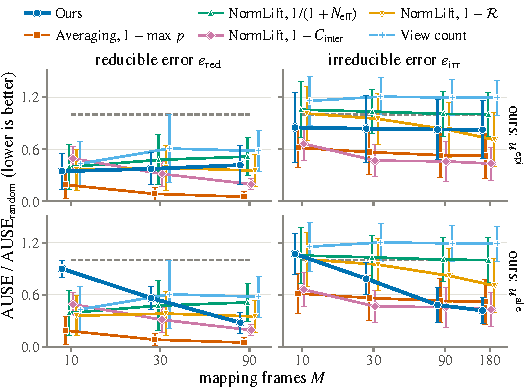
\includegraphics[width=\linewidth]{figs/views.pdf}
  \caption{Does each uncertainty rank its own error? AUSE divided by the AUSE
  of a random ranking of the same errors (dashed line; 0 is the oracle), for
  fields built from $M$ of the 180 mapping frames, against the reducible error
  $e_{\mathrm{red}}$ and the irreducible error $e_{\mathrm{irr}}$. Top: our
  $u^{\mathrm{epi}}$, bottom: our $u^{\mathrm{ale}}$, each with the same
  references. $M=180$ is the full map, where $e_{\mathrm{red}}$ is empty.
  Replica test, mean $\pm$ std over $N=6$ scenes.}
  \label{fig:views}
\end{figure}

Fig.~\ref{fig:views} tests whether the two channels separate. The references
are our total uncertainty, one minus the maximum probability of P2, the same
score for averaging, the view count $1/(1+n_{\mathrm{vis}})$ over views with
nonzero pixel mass, and NormLift's $1/(1+N_{\mathrm{eff}})$,
$1-C_{\mathrm{inter}}$ and $1-\mathcal{R}$. With few views,
$u^{\mathrm{epi}}$ ranks $e_{\mathrm{red}}$ better than $u^{\mathrm{ale}}$
(0.35 vs 0.90 at $M=10$, in all six scenes). With many views,
$u^{\mathrm{ale}}$ ranks $e_{\mathrm{irr}}$ better than $u^{\mathrm{epi}}$
(0.48 vs 0.83 at $M=90$, all six scenes; 0.42 vs 0.82 on the full map, five
of six). At $M=10$, $u^{\mathrm{ale}}$ is defined on only 4\% of the covered
pixels. The count-based scores rank $e_{\mathrm{irr}}$ close to random or
worse (on the full map 0.82 for our $u^{\mathrm{epi}}$, 1.00 and 1.19 for the
two counts): more views do not fix these errors. A total uncertainty ranks
$e_{\mathrm{red}}$ better than either channel alone. There ours and averaging
tie (0.19 at $M=10$), and on $e_{\mathrm{irr}}$ ours is lower than averaging
at every $M$ (0.44 vs 0.52 on the full map, all six scenes at $M=90$ and
180). The channels add what one score cannot: they tell the two kinds of
error apart. On $e_{\mathrm{irr}}$, $u^{\mathrm{ale}}$ is on par with
$1-C_{\mathrm{inter}}$ (0.42 vs 0.43 on the full map).

%% ----------------------------------------------------------------------------
\subsection{Real Object Removal: Stale Content}
\label{sec:exp-change}
\begin{table*}[t]
\centering
\caption{Stale-content detection on the object-removal test scenes (mean
$\pm$ std, $N=10$). AP, AUROC, FA and Rec.\ in \%. Input: I = image, D =
observed LiDAR depth, F = features. \reimpl Our re-implementation
(for~\cite{ackermann2025clsplats, jiang2026mif}, of the per-pixel feature
residual only). \textbf{Bold}: best, \underline{underline}: second best.
FA and Rec.\ at each row's own label-free threshold; the fused row has none.}
\label{tab:change}
\footnotesize
\setlength{\tabcolsep}{4pt}
\begin{tabular}{@{}llcccccc@{}}
\toprule
& & \multicolumn{2}{c}{Gaussian level} & \multicolumn{2}{c}{Pixel level}
& \multicolumn{2}{c}{Operating point}\\
\cmidrule(lr){3-4}\cmidrule(lr){5-6}\cmidrule(l){7-8}
Method & Input & AP$\uparrow$ & AUROC$\uparrow$ & AP$\uparrow$ & AUROC$\uparrow$
& FA$\downarrow$ & Rec.$\uparrow$\\
\midrule
%% generated by scripts/make_tables.py tab2 nor/tab2_relmax/change_test.json (test, N=10, run once);
%% log: docs/reports/2026-10-17-paper-completion/logs/nor_tab2_test.tex
NCC photometric residual & I & 30.4{\scriptsize$\,\pm\,$11.3} & 75.3{\scriptsize$\,\pm\,$13.5} & 48.0{\scriptsize$\,\pm\,$14.4} & 72.5{\scriptsize$\,\pm\,$8.0} & 12.4{\scriptsize$\,\pm\,$11.1} & 46.3{\scriptsize$\,\pm\,$28.8}\\
Depth residual & D & 57.4{\scriptsize$\,\pm\,$23.3} & 89.3{\scriptsize$\,\pm\,$5.6} & 39.7{\scriptsize$\,\pm\,$21.3} & 67.5{\scriptsize$\,\pm\,$14.2} & \underline{0.6}{\scriptsize$\,\pm\,$0.7} & 22.8{\scriptsize$\,\pm\,$23.5}\\
Feature residual, $k=2$~\cite{ackermann2025clsplats, jiang2026mif}\reimpl & F & 56.6{\scriptsize$\,\pm\,$23.3} & 87.6{\scriptsize$\,\pm\,$8.1} & 57.8{\scriptsize$\,\pm\,$22.2} & \underline{78.6}{\scriptsize$\,\pm\,$11.9} & 13.7{\scriptsize$\,\pm\,$7.1} & \textbf{75.6}{\scriptsize$\,\pm\,$22.7}\\
NormLift reliability drop~\cite{zang2026normlift}\reimpl & F & \underline{63.8}{\scriptsize$\,\pm\,$15.2} & \underline{91.6}{\scriptsize$\,\pm\,$4.6} & \textbf{65.8}{\scriptsize$\,\pm\,$14.3} & \textbf{82.0}{\scriptsize$\,\pm\,$9.4} & 4.1{\scriptsize$\,\pm\,$5.0} & 41.0{\scriptsize$\,\pm\,$39.6}\\
Dispersion $1-\hat\rho$ (ours) & F & 18.4{\scriptsize$\,\pm\,$8.4} & 53.2{\scriptsize$\,\pm\,$3.6} & 45.8{\scriptsize$\,\pm\,$23.8} & 66.4{\scriptsize$\,\pm\,$14.5} & \textbf{0.5}{\scriptsize$\,\pm\,$0.5} & 8.0{\scriptsize$\,\pm\,$9.0}\\
\midrule
Ours: test, reset, re-admission & F+D & 53.4{\scriptsize$\,\pm\,$22.5} & 87.2{\scriptsize$\,\pm\,$8.0} & 57.2{\scriptsize$\,\pm\,$20.3} & 77.8{\scriptsize$\,\pm\,$11.0} & 6.2{\scriptsize$\,\pm\,$5.1} & \underline{56.8}{\scriptsize$\,\pm\,$25.5}\\
Ours fused with depth residual & F+D & \textbf{75.0}{\scriptsize$\,\pm\,$12.9} & \textbf{92.3}{\scriptsize$\,\pm\,$2.9} & \underline{61.8}{\scriptsize$\,\pm\,$13.8} & 78.2{\scriptsize$\,\pm\,$11.3} & -- & --\\
\bottomrule
\end{tabular}
\end{table*}

Table~\ref{tab:change} reports stale-content detection. Before any reset,
our score differs from the feature-residual row only in where it takes the
cosine: per Gaussian against all of its earlier evidence, not per pixel
against the rendered map.
Ours also sets its threshold from the mapping pass, resets the Gaussians it
flags, and re-admits them after the depth check. The fused row asks whether
our score adds to the depth residual. In the test scenes, 27\% of the
Gaussians are seen by no update view and are not in the table. Our score adds
to depth: the fused row has the highest Gaussian-level AP and AUROC (75.0 and
92.3, against 57.4 and 89.3 for the depth residual alone). Alone, our test is
not the best ranking. NormLift's reliability drop ranks the stale Gaussians
better (AP 63.8 vs 53.4, higher in seven of ten scenes) and is the best row at
the pixel level (AP 65.8, AUROC 82.0). At its label-free threshold, our test
flags 56.8\% of the stale Gaussians at 6.2\% false alarms, against 75.6\% at
13.7\% for the feature residual and 22.8\% at 0.6\% for the depth residual.
After the update, 4.8\% of the stale Gaussians are still in our robust set.
The dispersion $1-\hat\rho$ alone does not detect a removal (AP 18.4).
Fig.~\ref{fig:qual} shows examples.

\begin{figure}[t]
  \centering
  \fbox{\parbox[c][0.45\linewidth][c]{0.92\linewidth}{\centering\footnotesize
  \todo{Qualitative figure. Top row: one object-removal validation frame
  after the removal. Bottom row: one Replica frame. Columns: image, query
  result, $u^{\mathrm{epi}}$, $u^{\mathrm{ale}}$, change score $\bar c$ with the
  flagged Gaussians.}}}
  \caption{Qualitative results. \todo{caption once the figure exists.}}
  \label{fig:qual}
\end{figure}

%% ----------------------------------------------------------------------------
\subsection{Ablations}
\label{sec:ablation}
%% Code switches for the rows (usplat/vmf_field.py FieldConfig):
%%  * Pixels instead of views: evidence="pixels", epistemic="pixels". With
%%    evidence="pixels" alone, u_epi would stay the Kish view count (review
%%    finding, check_ablation_switches.log).
%%  * Uncorrected mean length r-bar: estimator="rbar"; prior-shrunk: "joint";
%%    shrunk r-tilde: "legacy" (read-outs of the same sums, usplat/ablation_rows.py).
%%  * Full method: calib_mode="history" (history-conditioned null). Pooled
%%    null: calib_mode="pooled" (one quantile). Per-Gaussian max null: "max".
%%    Field states saved before 2026-09-29 called the history rule "pooled";
%%    from_state maps them to "history".
\begin{table}[t]
\centering
\caption{Ablations on the test scenes, mean over $N=6$ (top) and $N=10$
(bottom). Each row changes one part of the full method. AUSE: the row's
$u^{\mathrm{epi}}$ (epi) and $u^{\mathrm{ale}}$ (ale) against the 0/1 error
of the full map (the split into $e_{\mathrm{red}}$ and $e_{\mathrm{irr}}$ is
Fig.~\ref{fig:views}). AP at the Gaussian (G) and pixel (P) level. Kept: share of stale
Gaussians in the robust set after the update. All metrics except NLL in \%.
\todo{replace placeholders.}}
\label{tab:ablation}
\footnotesize
\setlength{\tabcolsep}{3.5pt}
\begin{tabular}{@{}lccccc@{}}
\toprule
\multicolumn{4}{@{}l}{\emph{Replica test}} & \multicolumn{2}{c}{AUSE$\downarrow$}\\
\cmidrule(l){5-6}
Variant & mIoU$\uparrow$ & ECE$\downarrow$ & NLL$\downarrow$ & epi & ale\\
\midrule
%% generated by scripts/make_tables.py tab3 tab3/eval_test.json --val tab3/eval_val.json
%% --tab1 tab1/eval_test.json (full method = ours_P2, lowest validation NLL; its cells
%% equal Table I's P2 row); log: docs/reports/2026-10-17-paper-completion/logs/tab3_rows.tex
\textbf{Full method} & 28.0 & 8.7 & 1.00 & 16.4 & 8.5\\
Pixels instead of views & 27.9 & 8.1 & 1.01 & 16.5 & 8.8\\
Uncorrected mean length $\bar r$ & 28.0 & 8.6 & 0.99 & 16.4 & 8.5\\
Prior-shrunk agreement & 28.0 & 8.5 & 1.01 & 16.4 & 14.8\\
Shrunk mean length $\tilde r$ & 28.0 & 8.7 & 1.00 & 16.4 & 8.5\\
Centered features & 28.0 & 8.6 & 0.99 & 16.4 & 8.3\\
Pixel-level variant & 27.9 & 8.1 & 1.01 & 16.5 & 8.8\\
\midrule
\emph{Object removal, test} & \multicolumn{2}{c}{AP$\uparrow$} & & &\\
\cmidrule(lr){2-3}
Variant & G & P & FA$\downarrow$ & Rec.$\uparrow$ & Kept$\downarrow$\\
\midrule
\textbf{Full method}            & \ph & \ph & \ph & \ph & \ph\\
No persistence ($k=1$)         & \ph & \ph & \ph & \ph & \ph\\
Persistence $k=\phn$           & \ph & \ph & \ph & \ph & \ph\\
Two buckets, $\lambda=\ph$     & \ph & \ph & \ph & \ph & \ph\\
Pooled null                    & \ph & \ph & \ph & \ph & \ph\\
Per-Gaussian max null          & \ph & \ph & \ph & \ph & \ph\\
Fixed threshold (val.)         & \ph & \ph & \ph & \ph & \ph\\
Re-admission without depth     & \ph & \ph & \ph & \ph & \ph\\
Centered features              & \ph & \ph & \ph & \ph & \ph\\
Pixel-level variant            & \ph & \ph & \ph & \ph & \ph\\
\bottomrule
\end{tabular}
\end{table}

In the Replica block of Table~\ref{tab:ablation}, \emph{Pixels instead of
views} uses the pixel masses
$m_{v,n}$ in place of $\omega_{v,n}$ in the posterior and the support, with
$u^{\mathrm{epi}}=1/(1+\sum_v m_{v,n})$. Its $\hat\rho$ still combines view
means, now with pixel-mass weights, since a pixel-level $Q$ would need an
extra render of squared weights. The agreement rows replace
$\hat\rho$~\eqref{eq:rho} by the uncorrected $\bar r$, by the prior-shrunk
$\lVert\R\rVert/(W_1+c_0)$, or by the shrunk mean length
$\tilde r=\bar r-(1-\bar r)/(W_1+1)$. Note that $\tilde r=1$ whenever
$\bar r=1$, so $\tilde r$ does not correct the one-view case. \emph{Centered
features} subtract the scene-mean feature before the dispersion and the
change test. The full method uses P2, the predictive with the lowest
validation NLL (Table~\ref{tab:replica}). On Replica only the agreement
read-out matters much. Shrinking the agreement with the prior raises the
aleatoric AUSE from 8.5 to 14.8, since it mixes the amount of evidence into
the aleatoric channel. The bias correction of $\hat\rho$ changes no cell by
more than 0.05 on the test or the validation scenes ($\bar r$ and $\tilde r$),
so these data do not show a benefit of the correction. Counting pixels instead
of views leaves mIoU and the epistemic AUSE unchanged and ranks errors slightly
worse (8.8). It lowers the test ECE (8.1 vs 8.7) but raised the validation ECE
(5.2 vs 4.9). Centering lowers the aleatoric AUSE a little on both splits (8.3
vs 8.5 on test, 4.7 vs 5.0 on validation). The bottom block uses the
object-removal scenes. The persistence and bucket rows vary $k$ and the retention $\lambda$ of
the change test. The threshold rows replace the history-conditioned null by
one pooled null per scene, by a null of per-Gaussian maxima over the mapping
pass, or by one fixed threshold from the validation scenes.
\emph{Re-admission without depth} re-admits a Gaussian after the views alone.
The \emph{pixel-level variant} turns every part off. It counts pixels, uses
$\tilde r$, has no change test, forgets by decaying the evidence of Gaussians
with low $\bar r$, and scores change by $1-\bar r$. We keep a part only if
removing it hurts on the validation scenes. \todo{interpret once
measured, then rename the method and adjust the claims to the parts that
remain.}

%% Run time and memory: the former Table IV is parked in parked_sections.tex.
%% Hardware from nvidia-smi and lscpu on the mapping machine (2026-09-29).
%% Keep it only if the timing runs on this machine.
\textbf{Run time and memory.} We time one validation scene per dataset on one
NVIDIA GeForce RTX 5070 Ti with an Intel Core i5-14600KF and no other job
running. On Replica (object removal), a keyframe takes \ph\ (\ph)\,ms in total: \ph\
(\ph)\,ms for LSeg feature extraction, \ph\ (\ph)\,ms for the render and
backward pass, and \ph\ (\ph)\,ms for the statistics, change test and
re-admission. Peak GPU memory is \ph\,GB. Averaging and NormLift reuse the
sums of our backward pass and add no render or backward pass. Fitting the 3D-GS
map takes \ph\,min per scene, and the field state takes \ph{} bytes per
Gaussian.

%% ----------------------------------------------------------------------------
\subsection{Limitations}
\label{sec:limitations}
The geometry is fixed after mapping, so moved content is not inserted at its
new place. The features limit the absolute accuracy: fusion cannot fix a class
that LSeg confuses in every view. The change statistic is a known residual
whose threshold assumes a static mapping sequence. Content that moves during
mapping raises it, and the mapping-pass scores are in-sample (the map and the
PCA are fit on those frames), so the false-alarm rate on a new sequence can
exceed the nominal rate. The 5\,cm depth check cannot keep out a thin removed
object, such as a book on a table. All baselines are our re-implementations
(LEGaussians on our features), and differences from the authors' code may
remain. The removal scenes have no class labels, so the predictive is evaluated
on synthetic data (Replica) only.

%% ============================================================================
\section{Conclusion}
\label{sec:conclusion}
%% ============================================================================
We presented an open-vocabulary semantic field for 3D Gaussian Splatting that
counts evidence in views and keeps little evidence and conflicting evidence
apart. A known feature residual, with a threshold from the map's own mapping
pass, drives the reset and the depth-checked re-admission of changed
Gaussians. \todo{one sentence with the main measured result on object
removal and one on Replica.} Future work should insert new geometry where content has moved
and test the field with other feature extractors.

%% ============================================================================
%% References: papers/ref.bib (BibTeX, IEEEtran style); ieeectl.bib holds only
%% the IEEEtran.bst control entry (written by the preamble on the first pass).
%% ============================================================================
\bibliographystyle{IEEEtran}
\bibliography{ref}

\end{document}
